\subsection{TRIGONOMETRIC FUNCTIONS}

If we compose the functions \(\cos\theta\) , \(\sin\theta\) , \(\tan\theta\) , \(\cot\theta\) (defined on A) with the homomorphism \(x\to\Im(x/a)\) of R onto A, the functions

\[
\cos \Im \left(\frac {x}{a}\right), \quad \sin \Im \left(\frac {x}{a}\right), \quad \tan \Im \left(\frac {x}{a}\right), \quad \cot \Im \left(\frac {x}{a}\right)
\]

so obtained are called respectively the cosine, sine, tangent and cotangent of the number \(x\) relative to the base \(a\) , and are written \(\cos_a x\) , \(\sin_a x\) , \(\tan_a x\) , \(\cot_a x\) . The mapping \(x \to \cos_a x + i \sin_a x\) is the composition of \(\theta \to \cos \theta + i \sin \theta\) and \(x \to \Im(x/a)\) , so that, from the definition of \(\cos \theta\) and \(\sin \theta\) in no. 2, we have the identity

\[
e \left(\frac {x}{a}\right) = \cos_ {a} x + i \sin_ {a} x,\tag{5}
\]

which is equivalent to

\[
\cos_ {a} x = \Re \left(e \left(\frac {x}{a}\right)\right), \quad \sin_ {a} x = \Im \left(e \left(\frac {x}{a}\right)\right),
\]

and also, by (4), equivalent to

\[
\cos_ {a} x = \frac {\mathrm{I}}{2} \left(e \left(\frac {x}{a}\right) + e \left(- \frac {x}{a}\right)\right), \quad \sin_ {a} x = \frac {\mathrm{I}}{2 i} \left(e \left(\frac {x}{a}\right) - e \left(- \frac {x}{a}\right)\right).
\]

Hence the identities

\[
\cos_ {b} x = \cos_ {a} \left(\frac {a x}{b}\right), \quad \sin_ {b} x = \sin_ {a} \left(\frac {a x}{b}\right).\tag{6}
\]

The only trigonometric functions which arise in branches of mathematics where numerical calculation is not involved are those relative to the base \(2\pi\) referred to above; these functions are denoted simply by \(\cos x\) , \(\sin x\) , \(\tan x\) , \(\cot x\) in place of \(\cos_{2\pi}x\) , \(\sin_{2\pi}x\) , \(\tan_{2\pi}x\) , \(\cot_{2\pi}x\) . For the purposes of numerical calculation, there are tables of the trigonometric functions corresponding to the bases a = 360 and a = 400; and the formulae (6) allow us to deduce the values of the trigonometric functions relative to any other base.

The relations recalled earlier between the cosines and sines of angles evidently give rise to the same relations between the cosines and the sines of the numbers which measure these angles; in particular, we have

\[
\begin{array}{r l} & {\cos_ {a} (x + y) = \cos_ {a} x \cos_ {a} y - \sin_ {a} x \sin_ {a} y,} \\ & {\sin_ {a} (x + y) = \sin_ {a} x \cos_ {a} y + \sin_ {a} y \cos_ {a} x,} \\ & {\cos_ {a} (- x) = \cos_ {a} x, \qquad \sin_ {a} (- x) = - \sin_ {a} x,} \\ & {\qquad \cos_ {a} ^ {2} x + \sin_ {a} ^ {2} x = 1.} \end{array}
\]

The functions \(\cos_{a}x\) and \(\sin_{a}x\) are continuous on R, and are periodic with period a; moreover, a is a principal period of these functions, for the relation \(\cos_{a}x = \cos_{a}y\) implies that either \(\sin_{a}x = \sin_{a}y\) or

\[
\sin_ {a} x = - \sin_ {a} y, \quad \text { i.e., }
\]

\[
e \left(\frac {x}{a}\right) = e \left(\frac {y}{a}\right) \quad \text { or } \quad e \left(\frac {x}{a}\right) = e \left(- \frac {y}{a}\right),
\]

so that either

\[
x \equiv y (\mathrm{mod} a) \quad \text { or } \quad x \equiv - y (\mathrm{mod} a);
\]

and similarly

\[
\sin_ {a} x = \sin_ {a} y
\]

is equivalent to either \(x \equiv y \pmod{a}\) or \(x + y \equiv \frac{1}{2} a \pmod{a}\) .

It follows from this that \(\cos_{a}x\) never takes the same value twice in the interval \([0,\frac{1}{2}a]\) ; hence, when restricted to this interval, it is a bijective mapping of this interval onto the interval \([-1,+1]\) . Since \(\cos_{a}0=1\) and \(\cos_{a}\left(\frac{1}{2}a\right)=-1\) , \(x\to\cos_{a}x\) is a strictly decreasing mapping of \([0,\frac{1}{2}a]\) onto \([-1,1]\) (Chapter IV, § 2, no. 6, Theorem 5 and Remark). We have \(\cos_{a}x=0\) for x=a/4, \(\cos_{a}x>0\) for \(0\leqslant x<a/4\) , \(\cos_{a}x<0\) for \(a/4<x\leqslant a/2\) . Since \(\cos_{a}(-x)=\cos_{a}x\) we can deduce how \(\cos_{a}x\) varies in the interval \([-\frac{1}{2}a,0]\) , and hence throughout the whole of R by periodicity (Fig. 8). Since \(\sin_{a}x=-\cos_{a}(x+a/4)\) we can also deduce how \(\sin_{a}x\) varies in R (Fig. 8).

\pandocbounded{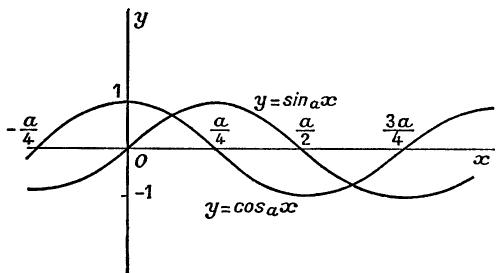
\includegraphics[keepaspectratio]{images/part001_7529c0a8.jpg}}\\
Figure 8.

The function \(\tan_{a}x\) is a continuous mapping of \(\mathbf{R}\) onto \(\tilde{\mathbf{R}}\) ; it takes the value \(\infty\) for the values \(\frac{1}{4} a + \frac{1}{2} ka\) ( \(k \in \mathbf{Z}\) ). Since \(\frac{1}{2} a\) is a period of \(\tan_{a}x\) , it is a principal period. In the interval \([0, \frac{1}{4} a]\) , \(\sin_{a}x\) increases from \(0\) to \(1\) , \(\cos_{a}x\) decreases from \(1\) to \(0\) , and therefore \(\tan_{a}x\) is strictly increasing in \([0, \frac{1}{4} a[\) and maps this interval onto \([0, +\infty[\) ; it follows that \(\tan_{a}x\) is strictly increasing in the interval \(]-\frac{1}{4}a,+\frac{1}{4}a[.\) and is a homeomorphism of this interval onto R (Fig. 9).

\pandocbounded{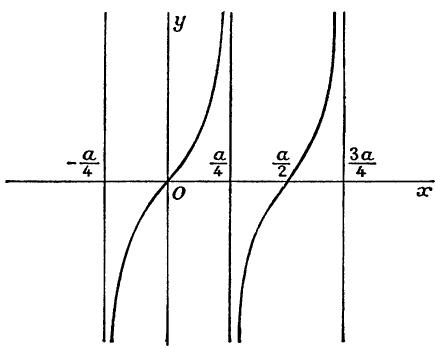
\includegraphics[keepaspectratio]{images/part001_329f289a.jpg}}\\
Figure 9.

